\documentclass{theme/uniprthesis}

%%%%%%%%%%%Some Extra Packages%%%%%%%%%%%
\usepackage[italian]{babel}		% To have Italina names in Sections, Figures, Chapters etc.
\usepackage{todonotes}			% To ease the revision



%%%%% THESIS / TITLE PAGE INFORMATION
% Everybody needs to complete the following:

\title{Addestramento di una rete neurale encoder-decoder con dati limitati per la segmentazione del femore fetale da immagini ecografiche}
\author{Dmitri Ollari Ischimji}
\advisor{Prof. Claudio Ferrari}
\college{Dipartimento di Ingegneria e Architettura}
\degree{Corso di Laurea Triennale in Ingegneria dei Sistemi Informativi}
\degreeyears{2023--2024}


% Not mandatory fields
\newcommand{\subTitle}{Training an encoder-decoder neural network with limited data for fetal femur segmentation from echographic images} %Subtitle, usually the english version of the title

%\newcommand{\advisorSecond}{Prof. Nome2 Cognome2} % For multiple (up to 4) advisors -- if this is not present then also the remaining ones are automatically omitted
%\newcommand{\advisorThird}{Dott. Nome3 Cognome3} % For multiple (up to 4) advisors -- if this is not present then also the remaining ones are automatically omitted
%\newcommand{\advisorFourth}{Dott. Nome4 Cognome4} % For multiple (up to 4) advisors

% \newcommand{\coadvisor}{Prof. co-Nome co-Cognome} %For multiple (up to 4) coadvisors -- if this is not present then also the remaining ones are automatically omitted
% \newcommand{\coadvisorSecond}{Prof. co-Nome2 co-Cognome2} % For multiple (up to 4) coadvisors -- if this is not present then also the remaining ones are automatically omitted
%\newcommand{\coadvisorThird}{Dott. co-Nome3 co-Cognome3} % For multiple (up to 4) coadvisors -- if this is not present then also the remaining ones are automatically omitted
%\newcommand{\coadvisorFourth}{Dott. co-Nome4 co-Cognome4} % For multiple (up to 4) coadvisors


\begin{document}

\maketitle

%%%% La dedica
\newpage
\thispagestyle{empty}
\null\vspace{\stretch{1}}
\begin{flushright}
	\textit{Dedicato a Diego}
\end{flushright}
\vspace{\stretch{3}}\null
\newpage

%%%% Gli indici
\pagestyle{plain}
\pagenumbering{arabic}
\tableofcontents
%
\listoffigures    %Commentare se non vi sono Immagini
% \listofalgorithms %Commentare se non vi sono Algoritmi
\listoftables     %Commentare se non vi sono Tabelle
%
%
%
%%%% La prefazione
% \chapter*{Introduzione} %Se si cambia il Titolo cambiare anche la riga successiva così che appia corretto nell'indice
\addcontentsline{toc}{chapter}{Introduzione} %Per far apparire Introduzione nell'indice (Il nome deve rispecchiare quello del chapter)
\pagenumbering{arabic} % Settaggio numerazione normale
L'introduzione deve contenere un riassunto del lavoro di Tesi.
In particolare bisogna esprimere chiaramente e molto sinteticamente: contesto dello studio, motivazioni, contributo e conclusioni.
Bisogna quindi fare un sommario dello studio ad alto livello, fornendo le intuizioni senza ricadere in dettagli tecnici.
Anche lo stile dovrebbe essere più discorsivo rispetto alle parti tecniche della tesi.


\chapter{Introduzione} \label{chap:Introduzione}

La segmentazione semantica riveste un ruolo cruciale nell'ambito dell'analisi
delle immagini mediche, consentendo di identificare e isolare strutture
anatomiche di interesse. Questa tesi si concentra sull'applicazione di reti
neurali convoluzionali (CNN) e, in particolare, sull'utilizzo dell'architettura
U-Net per eseguire la segmentazione binaria di immagini ecografiche fetali al
fine di estrarre e delineare i femori.

Le immagini ecografiche fetali rappresentano una sfida complessa nell'ambito
della segmentazione, richiedendo un'accurata identificazione delle strutture
anatomiche, come i femori, per fini diagnostici e monitoraggio della crescita
fetale. La segmentazione binaria semantica si concentra sull'etichettare pixel
specifici dell'immagine associati ai femori, consentendo una comprensione
dettagliata delle strutture anatomiche in esame.

L'approccio adottato in questa tesi si basa sull'utilizzo della rete neurale
convoluzionale U-Net, una struttura architetturale nota per la sua efficacia
nella segmentazione di immagini biomediche. La peculiarità di U-Net risiede
nella sua capacità di catturare dettagli locali mantenendo, allo stesso tempo,
una visione globale dell'immagine, rendendola particolarmente adatta per
problemi di segmentazione dettagliata come l'estrazione dei femori dalle
ecografie fetali.

Attraverso l'analisi, l'implementazione e l'ottimizzazione di questa
architettura, il lavoro si propone di migliorare l'accuratezza e l'efficienza
della segmentazione, fornendo uno strumento affidabile per l'identificazione
automatica dei femori nelle immagini ecografiche fetali. L'obiettivo è quello di
apportare un contributo positivo all'avanzamento delle tecnologie di estrazione
delle informazioni dalle immagini ecografiche fetali, automatizzando e
facilitando una valutazione più precisa della crescita fetale allo scopo di
analizzare la densità minerale ossea fetale(BMD).

%
%%%% I Capitoli di Contenuto	
\pagestyle{fancy}
  \chapter{Lavori correlati} \label{chap:related_works}
\section{Segmentazione} \label{sec:segmentazione}

\begin{figure}[!ht]
	\begin{center}
		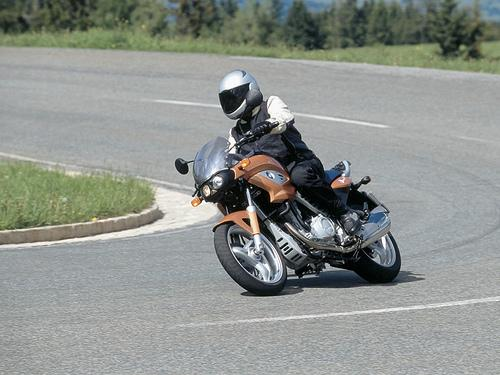
\includegraphics[width=0.4\textwidth]{Immagini/segmantion_example_image.png}
		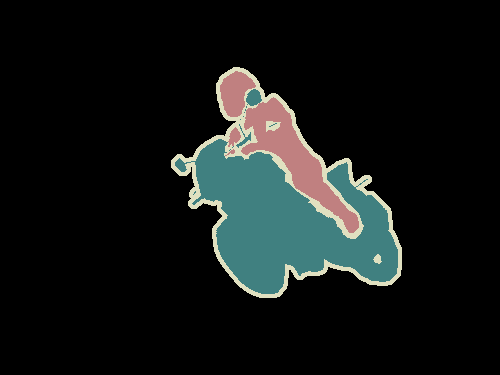
\includegraphics[width=0.4\textwidth]{Immagini/segmantion_example_mask.png}
	\end{center}
	\caption{Segmentazione semantica}
	\label{fig:segmentazione}
\end{figure}

La segmentazione semantica rappresenta un campo di grande interesse e rilevanza
nell'ambito dell'elaborazione delle immagini e della visione artificiale. Questa
tecnica si distingue per la sua capacità d'interpretare il contenuto delle
immagini a un livello semantico, andando oltre la semplice divisione
dell'immagine in regioni omogenee basate su caratteristiche visive come il
colore o la texture. Nello specifico, la segmentazione semantica si prefigge
l'obiettivo di attribuire un' etichetta semantica a ogni singolo pixel
dell'immagine, consentendo così d'identificare e categorizzare le diverse parti
che compongono la scena.  L'obiettivo principale della segmentazione semantica è
quello di fornire una comprensione approfondita del contenuto visivo presente in
un'immagine. Ciò si traduce nella capacità d'identificare e categorizzare
oggetti e regioni, rendendo possibile un'analisi dettagliata e una migliore
interpretazione dei dati visivi.
Un esempio di applicazione della segmentazione semantica la si pu\`o visionare
nella figura \ref{fig:segmentazione}, in questo caso l'obiettivo della segmentazione era quello di
estrapolare le informazioni relative al motociclista in una classe e le informazioni relative
al veicolo in un'altra classe, separando entrambe le classi dallo sfondo.


\section{Fully Convolutional Network}
\begin{figure}[!ht]
	\begin{center}
		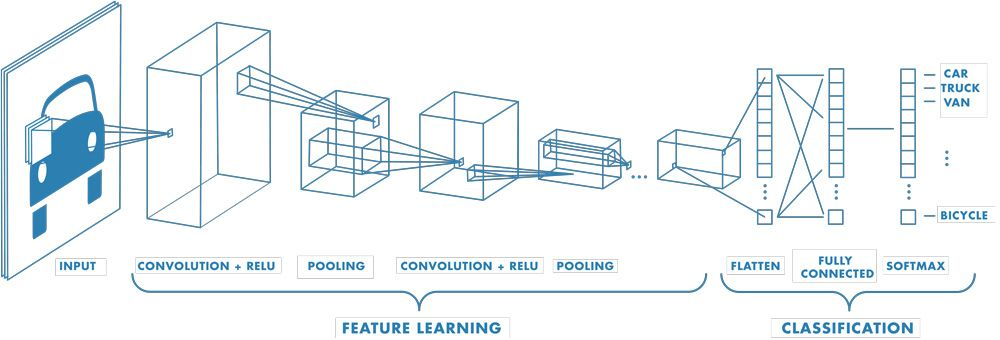
\includegraphics[width=0.8\textwidth]{Immagini/cnn.png}
	\end{center}
	\caption{CNN}
	\label{fig:cnn}
\end{figure}



\label{sec:fcn} L'articolo \textit{Fully
	Convolutional Networks for Semantic Segmentation} \cite{long2015fully} propone
l'utilizzo di una tipologia di reti neurali convoluzionali (CNN) che permettono
grazie all'assenza di layer completamente connessi di elaborare immagini di
qualunque dimensione. Questa nuova tipologia di reti migliora notevolmente le capacità di apprendimento delle reti neurali permettendo di produrre mappe
di segmentazione più precise grazie alla loro capacità di apprendimento d' informazioni spaziali.

Le motivazioni riguardanti l'ampio utilizzo nel settore della
\textit{computer vision} sono legate all'assenza di strati completamente
connessi (lineari) che vincolano l'ingresso alla medesima grandezza per ogni
singola immagine, permettendo di fornire in ingresso l'intera immagine e non
frammenti della stessa così da aumentare l'apprendimento spaziale della rete.

Questa maggior flessibilità comporta un addestramento libero da limitazioni
sull'ingresso comportando una maggiore tolleranza agli errori e al rumore
rendendo questa tipologia di reti particolarmente adatte a contesti poveri di
dati.

Le motivazioni per l'ampio utilizzo di queste reti nel settore della \textit{computer vision}
risiedono nell'assenza di strati completamente connessi, che solitamente vincolano l'ingresso a
dimensioni fisse per ogni immagine. Questa caratteristica permette alle reti di elaborare l'intera
immagine anziché solo frammenti, potenziando così l'apprendimento spaziale.

La maggiore flessibilità offerta da queste reti si traduce in un addestramento meno vincolato da
limitazioni dimensionali dell'input, risultando in una maggiore tolleranza agli errori e al rumore.
Di conseguenza, questa tipologia di reti si rivela particolarmente adatta in contesti caratterizzati
da una scarsità di dati.


\section{U-Net} \label{sec:unet}

\begin{figure}[!ht]
	\begin{center}
		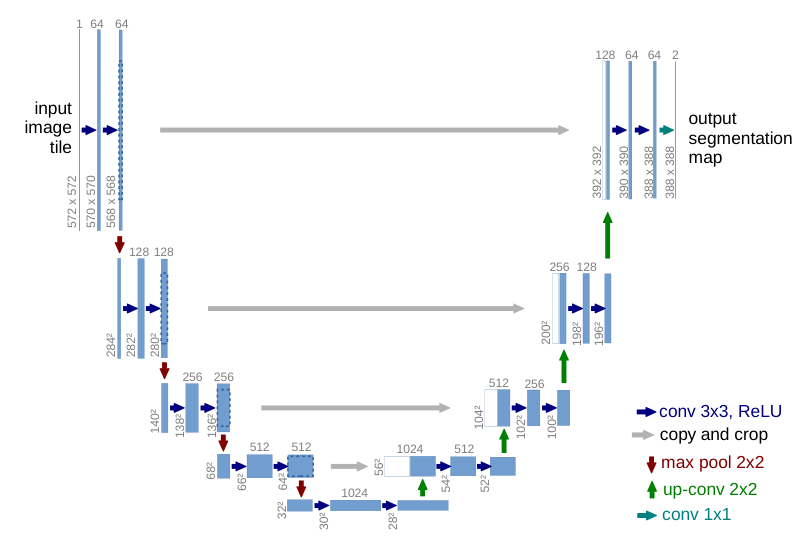
\includegraphics[width=0.8\textwidth]{Immagini/unet.png}
	\end{center}
	\caption{U-Net}\label{fig:unet}
\end{figure}


% \subsection{U-Net: Convolutional Networks for Biomedical Image Segmentation}
%
% Nel 2015, Olaf Ronneberger, Philipp Fischer e Thomas Brox hanno introdotto un nuovo modello di rete
% neurale convoluzionale chiamato \textit{U-Net} per la segmentazione semantica d'immagini biomedicali
% \cite{ronneberger2015unet}. Questa rete è stata progettata specificamente per affrontare le sfide
% associate alla segmentazione d'immagini biomedicali, come la necessità di segmentare strutture
% anatomiche precise con un numero limitato d'immagini di addestramento.
%
% Il modello \textit{U-Net} è caratterizzato da una struttura simmetrica, in cui la parte
% "contrattiva" (downsampling) cattura il contesto e la parte "espansiva" (upsampling) permette una
% localizzazione precisa. Questa struttura consente alla rete di combinare le informazioni di contesto
% con quelle locali, migliorando la precisione della segmentazione.
%
% Una delle principali innovazioni della \textit{U-Net} è l'introduzione di collegamenti a salti tra
% le parti contrattive ed espansive. Questi collegamenti trasferiscono le caratteristiche spaziali ad
% alta risoluzione dalla parte contrattiva a quella espansiva, consentendo una maggiore precisione
% nella localizzazione delle strutture segmentate.
%
% Il modello \textit{U-Net} ha dimostrato di ottenere risultati di segmentazione di alta qualità su
% diverse applicazioni biomedicali con un numero limitato d'immagini di addestramento, rendendolo uno
% strumento fondamentale per la segmentazione semantica in ambito biomedico.


\subsection{U-Net: Convolutional Networks for Biomedical Image Segmentation}

Nel 2015, Olaf Ronneberger, Philipp Fischer e Thomas Brox hanno introdotto il modello di rete
neurale convoluzionale \textit{U-Net} per la segmentazione semantica di immagini biomedicali
\cite{ronneberger2015unet}. Progettata specificatamente per affrontare le sfide della segmentazione
in ambito biomedico, come la necessità di segmentare con precisione strutture anatomiche con un
numero limitato di immagini di addestramento, U-Net ha rappresentato un notevole avanzamento.

Il modello \textit{U-Net} si distingue per una struttura simmetrica, dove la parte contrattiva
(downsampling) cattura il contesto e quella espansiva (upsampling) permette una localizzazione
precisa. Questa configurazione consente alla rete di fondere informazioni di contesto con quelle
locali, migliorando significativamente la precisione della segmentazione.

Una delle innovazioni chiave di \textit{U-Net} è l'introduzione di collegamenti a salti tra le parti
contrattive ed espansive, che trasferiscono caratteristiche spaziali ad alta risoluzione dalla parte
contrattiva a quella espansiva, aumentando la precisione nella localizzazione delle strutture
segmentate.

Grazie a queste caratteristiche, il modello \textit{U-Net} ha ottenuto risultati eccellenti nella
segmentazione di immagini biomedicali, anche con un numero limitato di immagini di addestramento,
diventando così un punto di riferimento nella segmentazione semantica biomedica.




\section{Segmentazione ossea} \label{sec:segmentazione_ossea}

Il lavoro \textit{Towards whole-body CT Bone Segmentation} \cite{10.1007/978-3-662-56537-7_59}
rappresenta un'importante analisi nello sviluppo di metodi e algoritmi avanzati per la segmentazione
ossea in immagini ottenute tramite tomografia computerizzata (TC) di tutto il corpo. Questo studio
pone l'accento sull'importanza della segmentazione ossea in campo medico, sia per la diagnosi di
condizioni patologiche sia per analisi dettagliate del tessuto osseo.

Il contributo fondamentale dell'articolo risiede nell'esplorazione di approcci innovativi e
nell'ottimizzazione di tecniche algoritmiche per identificare e isolare con precisione le strutture
ossee nelle immagini TC. Viene sottolineata l'importanza dell'uso di metodologie avanzate
nell'elaborazione delle immagini e dell'applicazione di algoritmi di visione artificiale e machine
learning per ottenere una segmentazione accurata.

L'articolo assume un ruolo significativo nel campo dell'informatica medica, evidenziando l'impiego
di soluzioni informatiche per un'analisi approfondita delle immagini mediche e riconoscendo
l'importanza delle tecniche di segmentazione ossea per applicazioni cliniche e di ricerca biomedica.


\section{Segmentazione di vasi sanguigni} \label{sec:segmentazione_vasi_sanguigni}

L'articolo \textit{Accurate Retinal Vessel Segmentation via Octave Convolution Neural Network}
\cite{fan2020accurate} introduce un approccio innovativo per la segmentazione precisa dei vasi
sanguigni retinici utilizzando le reti neurali a convoluzione ottava. Questa tecnica gioca un ruolo
cruciale nell'analisi delle immagini retiniche in ambito medico.

Il lavoro mette in luce i vantaggi offerti dalle reti neurali a convoluzione ottava, che utilizzano
differenti frequenze spaziali per catturare dettagli a diverse scale. Questo approccio risulta
particolarmente efficace nella segmentazione dei vasi sanguigni retinici, contribuendo
significativamente alla comprensione e diagnosi delle patologie oculari.

L'articolo dimostra l'efficacia di queste reti nel rilevare e isolare i vasi sanguigni della retina,
mostrando risultati più accurati rispetto ai metodi tradizionali. In definitiva, \textit{Accurate
	Retinal Vessel Segmentation via Octave Convolution Neural Network} offre un contributo importante
nel campo della segmentazione vascolare retinica, sottolineando l'efficacia e l'importanza delle
reti neurali a convoluzione ottava nella diagnostica medica.

  \chapter{Metodi} % (fold)
\label{cha:Metodi}

\section{Dati} % (fold)
Tutti i dati provengono da analisi ecografiche effettuate presso 
\textbf{Azienda Ospedaliera Universitaria Parma}, sono stati raccolti nel periodo compreso tra 
\textbf{Aprile 2022} e \textbf{Gennaio 2023} da un team di \textbf{medici esperti} e sono stati applicati
dei parametri per standardizzare le immagini raccolte:
\begin{itemize}
    \item Indice di massa corporea (BMI)
    \item Età
    \item Problematiche durante la gravidanza
    \item Problematiche dopo la gravidanza
    \item Femore centrato nell'inquadratura
\end{itemize}



Le immagini hanno subito un processo di \textit{preprocessing} aggiuntivo per
uniformare le dimensioni e la risoluzione. In particolare, sono state
ridimensionate a immagini \textbf{$1280px$ di larghezza} e \textbf{$876px$ di
altezza}.

Inoltre data che il problema è categorizzato come problema di segmantazione
semantica binomiale, si è scelto di convertire le immagine da \textbf{RGB} a
immagini in \textbf{scala di grigi} per ridurre la complessità del problema e
per ridurre il quantitativo di dati necessari per l'addestramento della rete.

Sono state realizzate manualmente delle \textbf{maschere} di segmantazione per
ogni immagine, in modo da avere un \textit{ground truth} da confrontare con le
predizioni del modello.

Data la scarsa quanti di dati a disposizione per l'addestramento della UNET, si è scelto di utilizzare alcune tecniche di \textit{data augmentation} per aumentare la quantità di dati a disposizione. In particolare si è scelto di utilizzare le seguenti tecniche applicate in modo casuale per ogni coppia \textbf{immagine-maschera}
\begin{itemize}
	\item \textit{Flip} orizzontale e verticale
	\item \textit{Rotazioni} di $35^{\circ}$
	\item \textit{Rumore} Gaussiano
\end{itemize}


Queste tecniche di \textit{data augmentation} migliorano notevolmente le
segmentazioni ottenute mediante la rete UNET e rendono la rete più robusta a
variazioni di luce e a rumore presente nelle immagini.


\begin{figure}
    \centering
    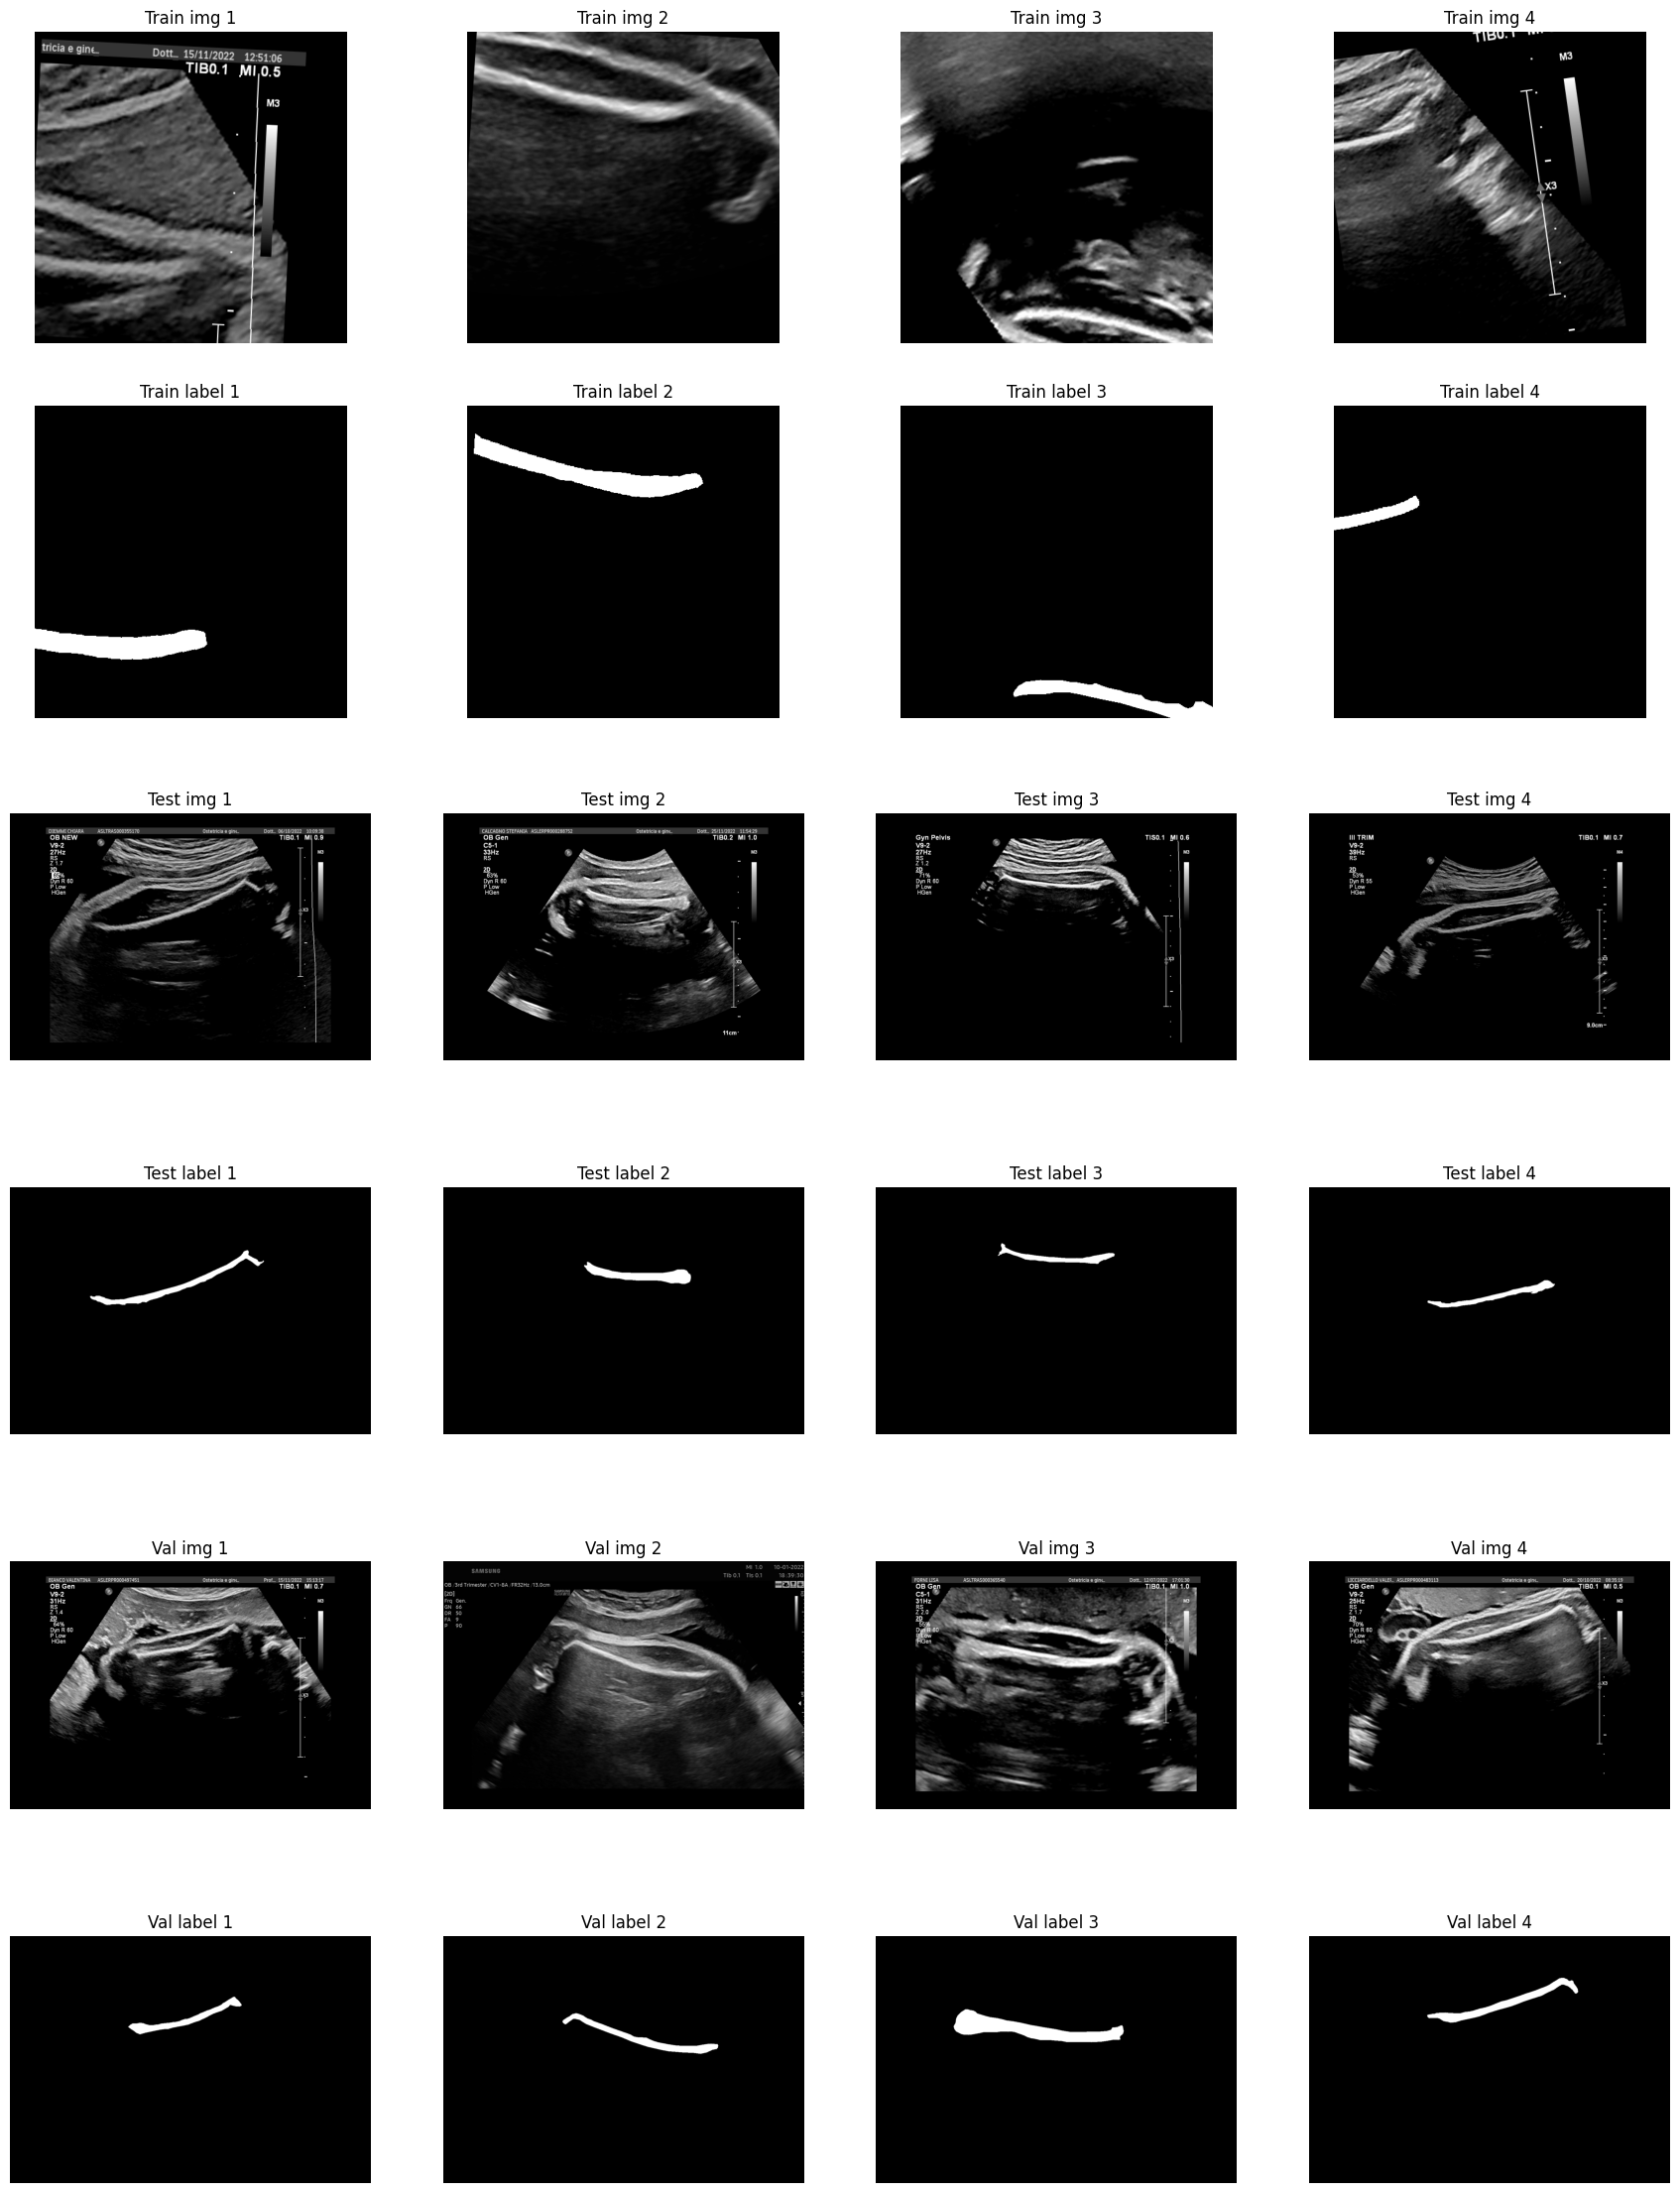
\includegraphics[width=0.8\textwidth]{Immagini/data_augmentation.png}
    \caption{Esempio di data augmentation}
    \label{fig:data_augmentation}
\end{figure}

L'ottimo risultato ottenuto è in buona parte dovuto alla \textit{data
augmentation} effettuata nella fase di addestramento del modello, la
\textit{data augmentation} ha migliorato l'adattabilità a contesti non
controllati migliorando così la generalizzazione del modello.

Come si può notare dalla \autoref{fig:data_augmentation} la \textit{data
augmentation} è stata effettuata in modo casuale per ogni coppia
\textbf{immagine-maschera} ed è stata applicata solo nella fase di
addestramento, lasciando cosi invariate le immagini inerenti al controllo del
modello.

\section{Etichettatura} Le immagini utilizzate per l'addestramento della rete
sono state fornite da \textbf{Azienda Ospedaliero-Universitaria di Parma} e sono
state etichettate manualmente mediante l'uso di un software di etichettatura
chiamato \textbf{LabelMe} \cite{labelme}.

Il processo di etichettatura della immagini prevede per ogni immagine
l'applicazione di indicatori che delimitano il perimetro del femore, potendolo
così isolare dal resto dell'immagine.





\section{Modello}

Il modello dal quale si è partiti prende il nome di
\textbf{U-Net}(\autoref{fig:unet}), la sua realizzazione iniziale è stata
effettuata seguendo lo studio di Olaf Ronneberger, Philipp Fischer e Thomas Brox
del 2015 \cite{ronneberger2015unet}.

Lo studio propone un'architettura di rete neurale convoluzionale per la
segmentazione semantica di immagini biomediche, classificando ogni singolo pixel
dell'immagine in una delle varie categorie del problema analizzato, la rete
convoluzionale emersa da quesa analisi rimane tutto'oggi una delle più
utilizzate in ambito medico per la segmentazione semantica data la sue
performace e la sua versatilità.

L'implementazione iniziale ricalca il modello realizzato da Olaf Ronneberger,
Philipp Fischer e Thomas Brox, utilizzando il framework \textbf{PyTorch}
\cite{pytorch} come base per la realizzazione della rete.



L'architettura proposta da Olaf Ronneberger, Philipp Fischer e Thomas Brox è
composta di 4 parti principali: \begin{itemize} \item \textbf{Encoder}:
Visionabile graficamente come la parte discenente della U-Net \item
\textbf{Bridge}: Visionabile graficamente come la linea di congiunzione fra la
parte discendente e la parte ascendente della U-Net \item \textbf{Decoder}:
Visionabile graficamente come la parte ascendente della U-Net \item
\textbf{Output}: Visionabile graficamente come l'ultimo layer della U-Net
\end{itemize}

Le applicazioni che si appogiano a modelli derivati dall'architettura U-net
dominano settori come la medicina e la biologia, in particolare la segmentazione
di immagini biomediche, come la segmentazione di immagini ecografiche, la
segmentazione di immagini TC e la segmentazione di immagini RM.

Le cause principali di tale successo possono essere ricondotte a:
\begin{itemize} \item \textbf{Segmentazione dettagliata}: U-Net è in grado di
produrre segmentazioni dettagliate e precise grazie alle sue innovative "skip
connections" che permettono al modello di catturare sia i dettagli di basso
livello che il contesto di alto livello.  \item \textbf{Architettura compatta}:
Nonostante la sua capacità di catturare dettagli, il modello è relativamente
snello e può essere addestrato con successo anche con dataset di dimensioni
moderate.  \item \textbf{Adattabilità}: U-Net è stata originariamente concepita
per applicazioni mediche, ma si è dimostrata estremamente versatile e può essere
utilizzata con successo in una vasta gamma di contesti.  \end{itemize}

Ovviamente, come ogni modello, U-Net ha anche alcuni svantaggi. Il principale è
la necessità di un dataset di addestramento ampio e accuratamente etichettato.
Questo aspetto può essere un ostacolo, soprattutto in contesti in cui la
disponibilità di dati è limitata. Inoltre, U-Net richiede una quantità
significativa di memoria per memorizzare i pesi del modello, il che può
diventare un problema quando si lavora con immagini ad alta risoluzione.




\subsection{Convoluzione} % (fold)
\label{sec:convoluzione}


La convoluzione è una delle operazini fondamentali utilizzate nelle reti neurali convoluzionali per estrarre le caratteristiche significative da un'input, la convoluzione coinvolge un filtro (o kernel) e l'input su cui si applica.

Il processo di convoluzione consiste nell'sommare ogni elemento di un'immagine al suo vicino, pesando ogni singola operazione mediante l'utilizzo del filtro(o kernel) il calcolo della feature map di uscita è calcolata come segue:
\begin{align}
  &\Bigg( \begin{bmatrix}
    a & b & c \\
    d & e & f \\
    g & h & i
  \end{bmatrix}
  *
  \begin{bmatrix}
    1 & 2 & 3 \\
    4 & 5 & 6 \\
    7 & 8 & 9
  \end{bmatrix}
  \Bigg) [2, 2] =\\
  &= (i \cdot 1) + (h \cdot 2) + (g \cdot 3) + (f \cdot 4) + ( e \cdot 5 ) + ( d \cdot 6 ) + c \cdot 7) + (b \cdot 8) + (a \cdot 9)
\end{align}


% subsection convoluzionale (end)

\subsection{Max pooling} % (fold)
\label{sec:Max pooling}
Il \textit{max pooling} è un'operazione chiave all'interno della rete U-Net e delle reti neurali convoluzionali (CNN) in generale.

Il \textit{max pooling} è utilizzato per ridurre la dimensione delle feature map, consentendo di ridurre la complessità del problema da approssimare, comportando una maggior resistenza all'\textit{overfitting}, migliorando la capacit\'a di generalizzazione del modello e di ottenere una rappresentazione più invariante rispetto alle piccole variazioni spaziali nell'input.





\subsection{Encoder} % (fold)
\label{sec:Encoder}

\todo{immagini encoder}


La fase di \textit{encoding} è la prima fase della rete U-Net, composta da una serie di strati di convoluzione(\ref{sec:convoluzione}) e max pooling(\ref{sec:Max pooling}) che riducono progressivamente la dimensione spaziale dell'immagine mentre aumentano il numero di canali di \textit{features}.

Nello specifico, la fase di \textit{encoding} è composta da 3 parti principali:
\begin{itemize}
  \item \textbf{Strato iniziale}: Questo strato applica diverse operazioni di convoluzione ai dati di input per estrarre le caratteristiche di basso livello, come bordi e texture. Queste operazioni iniziali consentono al modello di comprendere dettagli fondamentali dell'immagine.
  \item \textbf{Downsampling}: Dopo lo strato iniziale, la fase di encoding utilizza operazioni di max pooling o convoluzione con un passo (stride) superiore a 1 per ridurre la dimensione delle feature map. Questo processo di downsampling riduce la risoluzione spaziale, ma aumenta il numero di canali delle feature, catturando informazioni di livello superiore. Ogni strato di downsampling estrae caratteristiche sempre più astratte e globali dall'immagine.
  \item \textbf{Strati intermedi}: Nel cuore della fase di encoding si trovano gli strati intermedi. Questi strati applicano operazioni di convoluzione multiple con l'obiettivo di catturare caratteristiche di complessità crescente. A ogni strato intermedio, le feature map si allargano, consentendo al modello di comprendere dettagli più ampi e contestuali. Questi strati intermedi sono cruciali per l'acquisizione di informazioni di alto livello.
\end{itemize}

% subsection Encoder (end)





\subsection{Bridge} % (fold)
\label{sec:Bridge}
\todo{immagini bridge}

Il \textit{bridge} è un'innovazione dell'architettura U-Net che contribuisce in modo significativo alla precisione della segmentazione delle immagini.

La fase di \textit{bridge} permette di trasferire informazioni rilevanti tra l'encoder e il decoder attraverso skip connections, che consentono il trasferimento di informazioni rilevanti. Questo approccio multi-scala è fondamentale per ottenere una segmentazione precisa delle immagini, poiché consente al modello di considerare dettagli sia di basso che di alto livello durante il processo di segmentazione.



% subsection Bridge (end)

\subsection{Decoder} % (fold)
\label{sec:Decoder}

\todo{immagini decoder}
Nella rete U-Net, la fase di decoding \'e responsabile della ricostruzione dell'immagine segmentata a partire dalle informazioni estratte durante l'encoding. Questa fase \'e fondamentale per ottenere una segmentazione di alta qualit\'a.

Le fasi principali del \textit{decoder} sono:
\begin{itemize}
  \item \textbf{Upsampling}: La fase di decoding inizia con l'operazione di upsampling, che serve a ripristinare gradualmente la dimensione delle feature map ai livelli originali dell'immagine. Ciò viene fatto utilizzando operazioni come la trasposta della convoluzione (deconvoluzione) o l'interpolazione bilineare. L'obiettivo è ottenere feature map di dimensioni compatibili con quelle dell'immagine di input.
  \item \textbf{Skip Connections}: Un aspetto distintivo della U-Net sono le skip connections, o connessioni di salto. Queste connessioni collegano le feature map estratte durante l'encoding alle corrispondenti feature map nella fase di decoding. Ciò consente di combinare informazioni multi-scala, in modo che il modello possa accedere sia a dettagli fini che a contesto di alto livello. Le skip connections sono fondamentali per migliorare la precisione della segmentazione.
  \item \textbf{Convoluzione nel Decoding}: Dopo l'upsampling e l'integrazione delle skip connections, vengono applicate operazioni di convoluzione per raffinare ulteriormente le feature map. Queste convoluzioni possono avere lo scopo di "mescolare" le informazioni o di catturare dettagli specifici a livelli più alti.
\end{itemize}

% subsection Decoder (end)

\subsection{Output} % (fold)
\label{sec:Output}
La parte finale della rete U-Net \'e composta da uno o più strati di convoluzione che riducono la profondità delle feature map alla dimensione desiderata per l'output finale. Questi strati producono l'immagine segmentata in cui ogni pixel è etichettato con la classe di appartenenza (esempio: sfondo, oggetto, ecc.).

% subsection Output (end)

\section{Rimozione sliding window} % (fold)
\label{sub:Rimozione sliding window}
Grazie agli avanzamenti tecnologici portati avanti negli anni da costruttori hardware e software, si è riusciti a ridurre notevolmente i tempi di elaborazione delle immagini e la grandezza massima delle immagini che possono essere elaborate.

Si è quindi scelto di rinunciare all'approccio sliding window che risulta più conservativo in termini di memoria e di tempo di elaborazione, per un approccio più moderno che sfrutta la potenza di calcolo delle GPU e la loro memoria dedicata notevolmente più grande rispetto alle GPU del passato.

Un \textit{effetto collaterale} riscontrato con l'utilizzo di immagini intere è quello della miglior comprensione spaziale delle immagini da parte della rete, questo effetto è dovuto al fatto che la rete ha a disposizione l'intera immagine e non solo una parte di essa, questo permette alla rete di comprendere meglio il contesto spaziale dell'immagine e di migliorare la segmentazione.

% section Rimozione sliding window (end)



\section{Modifica Encoder-Decoder}

Mediante svariate prove si è notato che aumentando il numero di iterazioni di convoluzione nei vari strati di encoding e decoding, si ottengono risultati migliori in termini di segmentazione a scapito di un aumento del tempo di elaborazione e del consumo di memoria.

Si è quindi scelto di modificare le fasi di \textit{decoding} e di \textit{encoding}:

\begin{table}[H]
    \centering
        \begin{tabular}{|c|c|c|}
            \hline
            \textbf{Layer} & \textbf{In channels} & \textbf{Out channels} \\
            \hline
            \hline
            Encoder        & 1                    & 64                    \\
            \hline
            Encoder        & 64                   & 128                   \\
            \hline
            Encoder        & 128                  & 256                   \\
            \hline
            Encoder        & 256                  & 512                   \\
            \hline
        % \end{tabular}
        % \\
        
        % \begin{tabular}{|c|c|c|}
        %     \hline
            % \textbf{Layer} & \textbf{In channels} & \textbf{Out channels} \\
            % \hline
            Decoder        & 1024                 & 512                   \\
            \hline
            Decoder        & 512                  & 256                   \\
            \hline
            Decoder        & 256                  & 128                   \\
            \hline
            Decoder        & 128                  & 64                    \\
            \hline
        \end{tabular}
    \caption{Encoding e Decoding originale}
    \label{tab:encoding_originale}
\end{table}



\begin{table}[H]
    \centering
			\begin{tabular}{|c|c|c|}
				\hline
				\textbf{Layer} & \textbf{In channels} & \textbf{Out channels} \\
				\hline
				\hline
				Encoder        & 1                    & 16                    \\
				\hline
				Encoder        & 16                   & 32                    \\
				\hline
				Encoder        & 32                   & 64                    \\
				\hline
				Encoder        & 64                   & 128                   \\
				\hline
				Encoder        & 128                  & 256                   \\
				\hline
				Encoder        & 256                  & 512                   \\
				\hline
				Decoder        & 1024                 & 512                   \\
				\hline
				Decoder        & 512                  & 256                   \\
				\hline
				Decoder        & 256                  & 128                   \\
				\hline
				Decoder        & 128                  & 64                    \\
				\hline
				Decoder        & 64                   & 32                    \\
				\hline
				Decoder        & 32                   & 16                    \\
				\hline
		\end{tabular}
	\caption{Encoding e Decoding modificati}
	\label{tab:encoding_modificato}
\end{table}






L'idea alla base di questa modifica risiede nel significato intrinseco dell'operazione di convoluzione e di max pooling, 
aggiungendo iterazioni di convoluzioni, si permette alla rete in primo 
luogo di estrarre più feature importanti alla classificazione dei pixel e successivamente mediante il max pooling
si eliminano le feature meno importanti e si riduce la dimensione delle feature map.



% section Modifica encoding e decoding (end)



\section{Metriche}
\label{sec:metriche}

Considerando la tipologia di \textit{task} si è pensato di usare la metrica \textit{Dice BCE Loss} per la \textit{loss} e \textit{Intersection over Union} per l'\textit{accuratezza}.

\subsection{Dice BCE Loss}
La \textit{Dice BCE Loss} è una metrica che combina due metriche, la \textit{Dice Loss} e la \textit{BCE Loss}.

\begin{align}
	% \text{DiceBCELoss} &= \text{DiceLoss} + \text{BCELoss}
	L & = L_{\text{Dice}} + L_{\text{BCE}}
	\label{eq:dice_bce_loss}
\end{align}

\begin{align}
	L_{\text{Dice}} & = 1 - \frac{2\sum_i^N p_i g_i + \varepsilon}{\sum_i^N p_i^2 + \sum_i^N g_i^2 + \varepsilon}
	\label{eq:dice_loss}
\end{align}

\begin{align}
	L_{\text{BCE}} & = -\frac{1}{N} \Bigg[ g_i \sum_{i=1}^N p_i + ( 1 - g_i ) \sum_{i=1}^N (1-p_i) \Bigg]
	\label{eq:bce_loss}
\end{align}

Quindi ne risulta che la \textit{loss} sarà calcolata mediante:
\begin{align}
	L & = 1 - \frac{2\sum_i^N p_i g_i + \varepsilon}{\sum_i^N p_i^2 + \sum_i^N g_i^2 + \varepsilon} -\frac{1}{N} \Bigg[ g_i \sum_{i=1}^N p_i + ( 1 - g_i ) \sum_{i=1}^N (1-p_i) \Bigg]
	\label{eq:dice_bce_loss_complete}
\end{align}
Dove:
\begin{itemize}
	\item $p_i$ è il valore di \textit{ground truth}
	\item $g_i$ è il valore \textit{predetto} dal modello
\end{itemize}

\subsection{Intersection over Union(IoU)}
Per la metrica dell'accuratezza della segmentazione, è stata utilizzata la metrica \textit{Intersection over Union} (IoU),
poichè è una metrica che permette di valutare la capacità di segmentazione del modello
facendo il rapporto tra l'area di intersezione tra la maschera predetta e quella di \textit{ground truth} e l'area di unione tra le due maschere, formalmente:
\begin{align}
	\text{IoU} & = \frac{\text{TP}}{\text{TP} + \text{FP} + \text{FN}}
	\label{eq:iou}
\end{align}

Dove \textbf{TP} è il numero di \textit{True Positive}, \textbf{FP} è il numero di \textit{False Positive} e \textbf{FN} è il numero di \textit{False Negative}.

\section{Validazione del modello}

La \textit{cross-validation} (validazione incrociata) è una tecnica fondamentale nell'ambito del machine learning e dell'addestramento di modelli predittivi. Essenzialmente, la cross-validation è un metodo per valutare le prestazioni di un modello in modo robusto, valutandolo su più insiemi di dati per ottenere stime più affidabili delle sue capacità predittive. Questo processo aiuta a mitigare il rischio di overfitting (sovradattamento) e offre una migliore comprensione delle prestazioni del modello.


\begin{figure}[H]
    \centering
    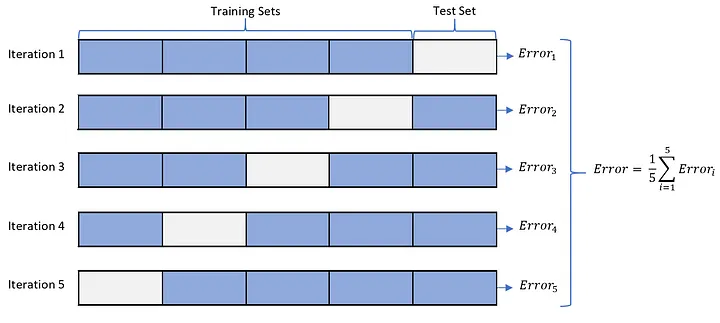
\includegraphics[width=0.7\textwidth]{Immagini/cross_validation.png}
    \caption{Cross-validation}
    \label{fig:cross_validation}
\end{figure}

Fornisce stime più affidabili delle prestazioni del modello, riducendo il rischio di ottenere stime di prestazioni spurie a causa di una singola divisione dei dati.




% chapter Metodi (end)
  \chapter{Risultati sperimentali} % (fold)
\label{chap:Risultati sperimentali}

\section{Addestramento} % (fold)
\label{sec:Addestramento}

Il modello \`e stato addestrato mediante l'uso della \textit{cross-validation}(\autoref{fig:cross_validation})
con una suddivisione dei dati in cinque parti uguali(cinque folds).

Essendo una tipologia di apprendimento supervisionata, al modello sono fornite immagini
originali e le loro segmentazioni effettuate manualmente.

\begin{figure}[h!]
    \centering
    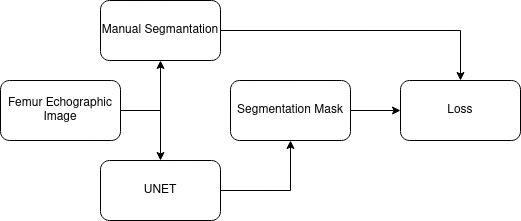
\includegraphics[width=0.7\columnwidth]{Immagini/training.png}
    \caption{Addestramento del modello}
    \label{fig:addestramento del modello}
\end{figure}


Effettuando l'addestramento con 5 folds, il modello viene addestrato 5 volte, ogni volta con un fold diverso,
l'errore finale \`e dato dalla media degli errori ottenuti dalle 5 iterazioni.

\begin{figure}[h!]
    \centering
    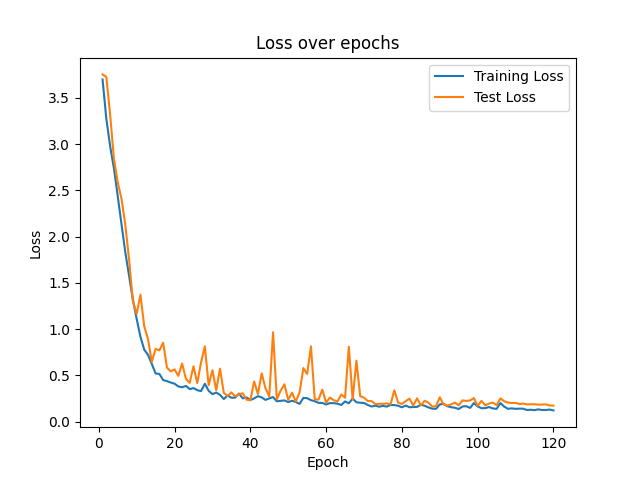
\includegraphics[width=0.4\columnwidth]{Immagini/fold_0_loss.png} 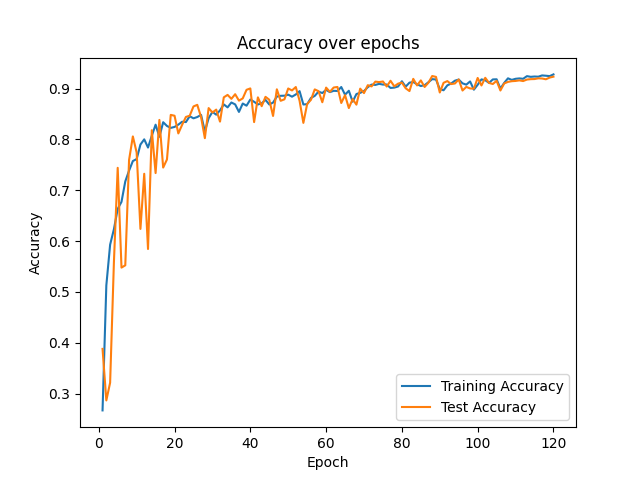
\includegraphics[width=0.4\columnwidth]{Immagini/fold_0_accuracy.png}
    \caption{Errore e accuratezza della prima porzione di dati}
    \label{fig:loss e accuratezza della prima porzione di dati}
\end{figure}

\begin{figure}
    \centering
    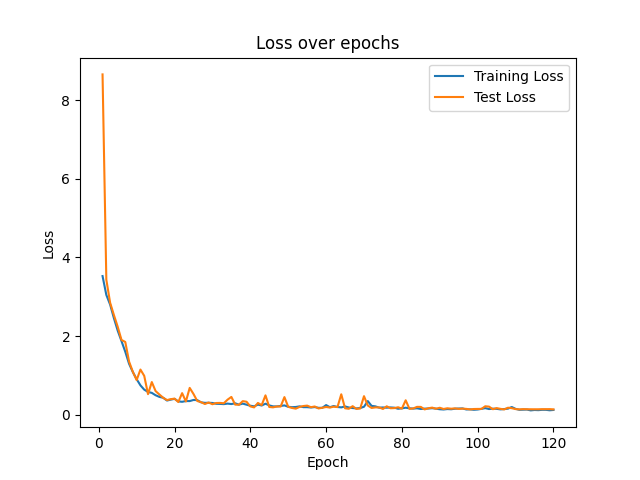
\includegraphics[width=0.4\columnwidth]{Immagini/fold_1_loss.png} 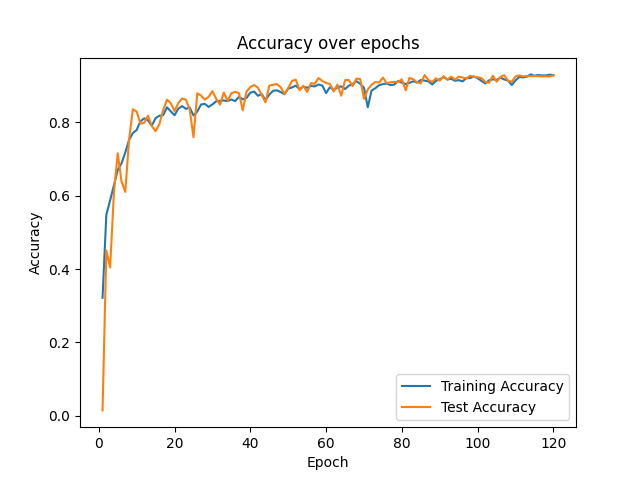
\includegraphics[width=0.4\columnwidth]{Immagini/fold_1_accuracy.png}
    \caption{Errore e accuratezza della seconda porzione di dati}
    \label{fig:loss e accuratezza della seconda porzione di dati}
\end{figure}

\begin{figure}
    \centering
    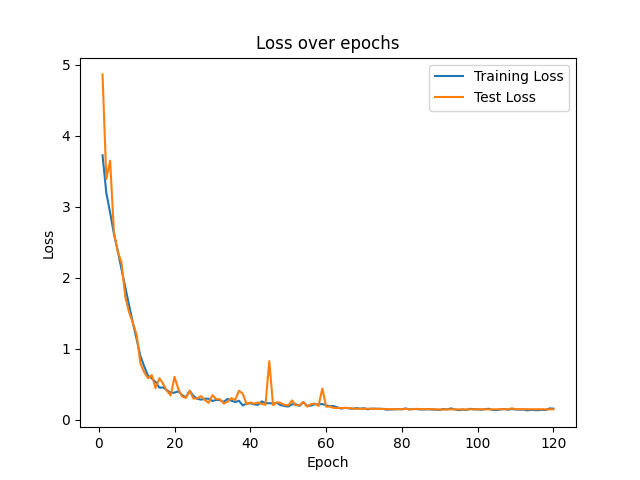
\includegraphics[width=0.4\columnwidth]{Immagini/fold_2_loss.png} 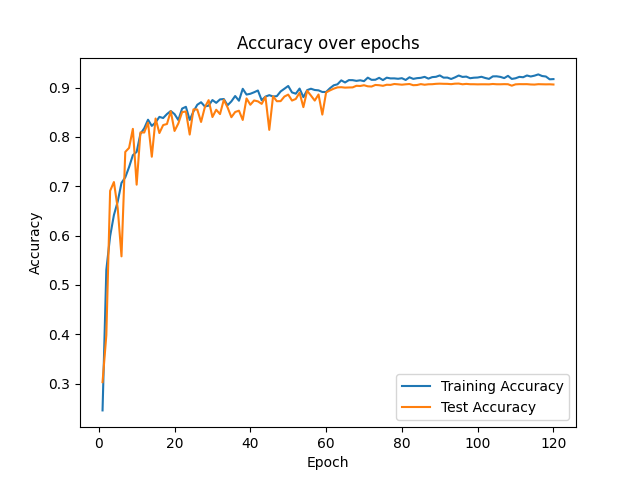
\includegraphics[width=0.4\columnwidth]{Immagini/fold_2_accuracy.png}
    \caption{Errore e accuratezza della terza porzione di dati}
    \label{fig:loss e accuratezza della terza porzione di dati}
\end{figure}

\begin{figure}
    \centering
    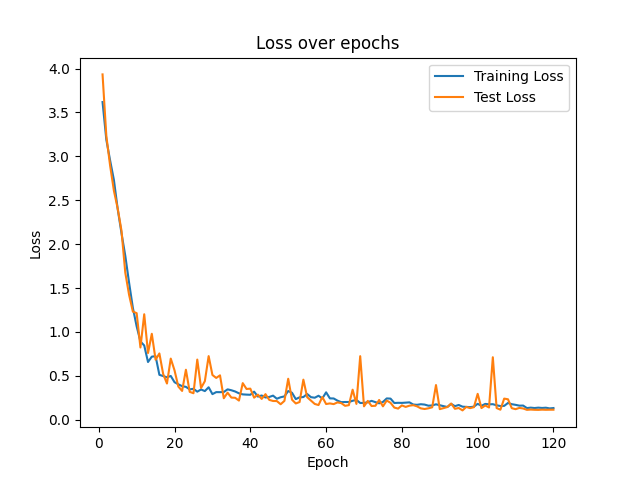
\includegraphics[width=0.4\columnwidth]{Immagini/fold_3_loss.png} 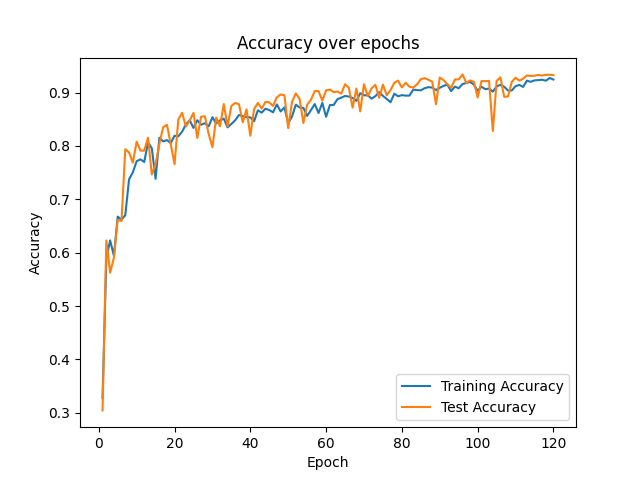
\includegraphics[width=0.4\columnwidth]{Immagini/fold_3_accuracy.png}
    \caption{Errore e accuratezza della quarta porzione di dati}
    \label{fig:loss e accuratezza della quarta porzione di dati}
\end{figure}

\begin{figure}
    \centering
    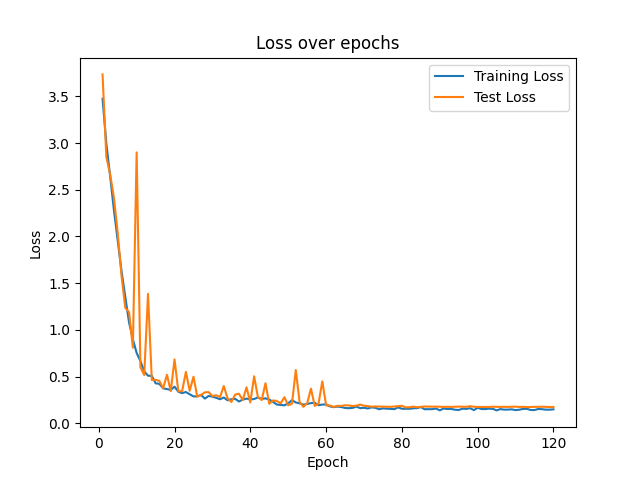
\includegraphics[width=0.4\columnwidth]{Immagini/fold_4_loss.png} 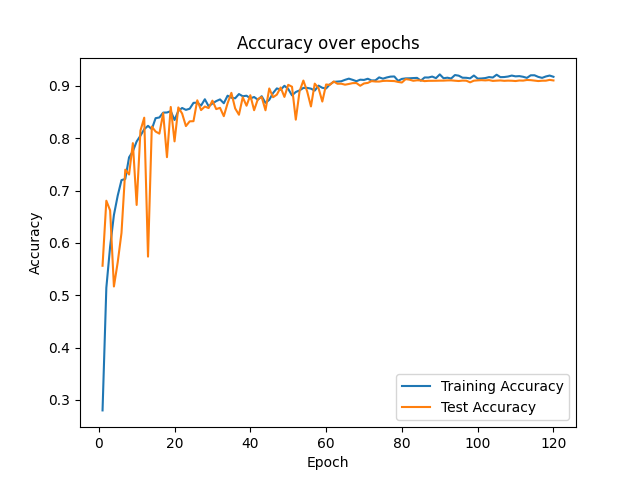
\includegraphics[width=0.4\columnwidth]{Immagini/fold_4_accuracy.png}
    \caption{Errore e accuratezza della quinta porzione di dati}
    \label{fig:loss e accuratezza della quinta porzione di dati}
\end{figure}

L'\textbf{errore} complessivo viene calcolato come media dei singoli errori
ottenuti dalle cinque iterazioni mediante la formula
\ref{eq:dice_bce_loss_complete} portando a un errore medio del
\textbf{$7.9\%$}.

Mentre l'\textbf{accuratezza} complessiva viene calcolata come media delle singole accuratezze
ottenute dalle cinque iterazioni mediante la formula \ref{eq:iou} portando a un'accuratezza media del \textbf{$92.1\%$}.




Considerando che questo modello \`e stato utilizzato in ambito medico per velocizzare e standardizzare 
la segmentazione dei femori per un'analisi su questi ultimi, oltre ad analisi quantitative, \`e stato 
necessario effettuare delle analisi qualitative sulla segmentazione ottenuta dal modello.

Nelle immagini seguenti viene riportato uno delle immagini prese in considerazione per l'addestramento del modello
e vengono mostrate le segmentazione manuali, le segmentazioni ottenute dal modello e la differenze 
nella classificazione dei pixel tra le due segmentazioni.





Partendo da una immagini (\autoref{fig:immagine originale}) ottenuta mediante la raccolta dati effettuata dai medici, 

\begin{figure}[h!]
    \centering
    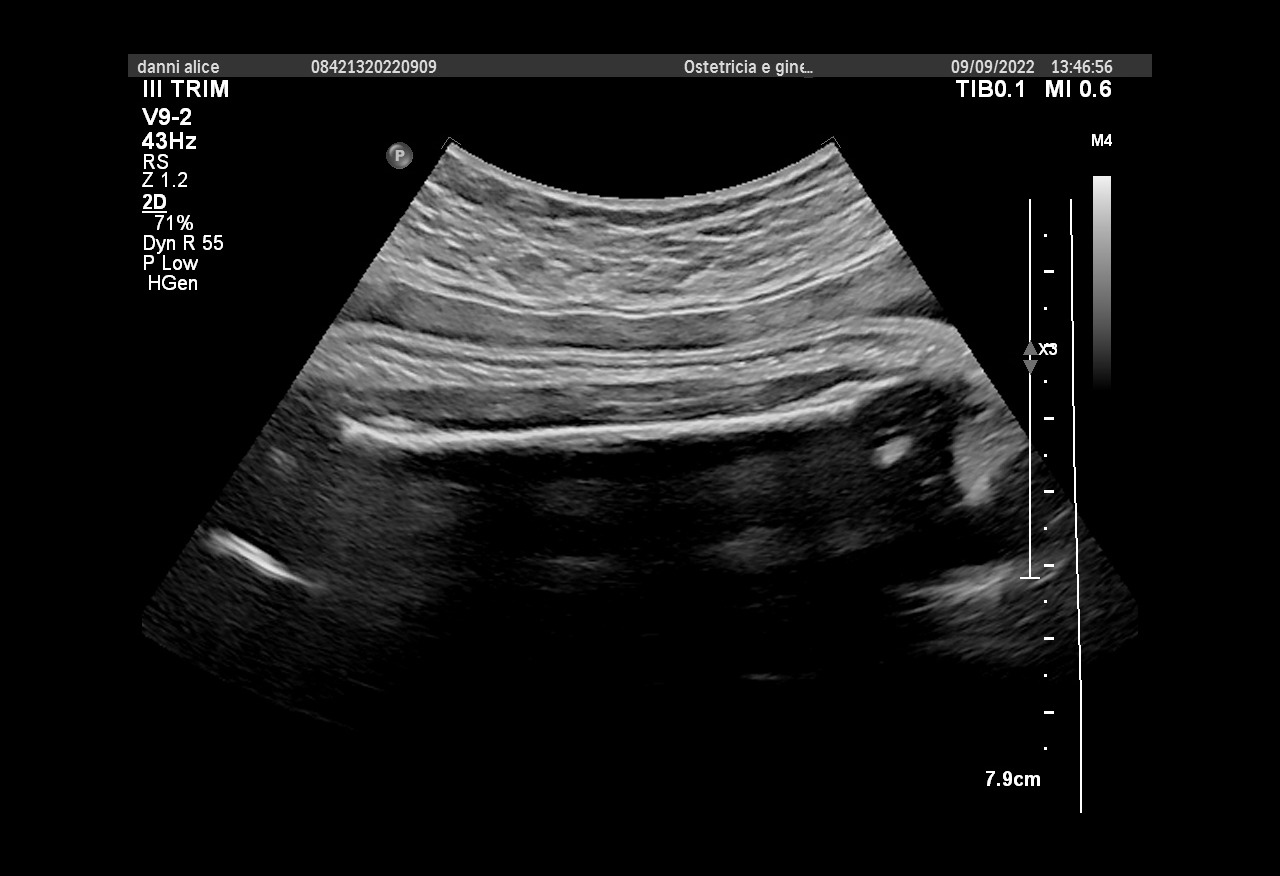
\includegraphics[width=0.7\columnwidth]{Immagini/image.png}
    \caption{Immagine originale}
    \label{fig:immagine originale}
\end{figure}


% I risultati ottenuti mediante la segmentazione manuale e la segmentazione del modello sono 
% rispettivamente \autoref{fig:segmentazione manuale} e \autoref{fig:segmentazione del modello}.

% \begin{figure}[h!]
%     \centering
%     
\includegraphics[width=0.4\columnwidth]{Immagini/mask.png}
%     \caption{Segmentazione manuale}
%     \label{fig:segmentazione manuale}
% \end{figure}

% \begin{figure}[h!]
%     \centering
%     
\includegraphics[width=0.4\columnwidth]{Immagini/prediction.png}
%     \caption{Segmentazione del modello}
%     \label{fig:segmentazione del modello}
% \end{figure}

\begin{figure}[h!]
    \centering
    \begin{minipage}{0.4\columnwidth}
        \centering
        
\includegraphics[width=\linewidth]{Immagini/mask.png}
        \caption{Segmentazione manuale}
        \label{fig:segmentazione manuale}
    \end{minipage}
    \hfill
    \begin{minipage}{0.4\columnwidth}
        \centering
        
\includegraphics[width=\linewidth]{Immagini/prediction.png}
        \caption{Segmentazione del modello}
        \label{fig:segmentazione del modello}
    \end{minipage}
\end{figure}

Per sostenere la tesi che il modello riesca a segmentare correttamente le immagini, \`e stata 
calcolata la distribuzione dei pixel per confrontare la segmentazione manuale con quella del modello.

% Per quantifica la differenza tra le due segmentazioni \`e stata calcolata la distribuzione dei pixel
% nelle immagini processate manuale e si \`e confrontata con la distribuzione dei pixel nelle immagini
% processate dal modello

% \begin{figure}[h!]
%     \centering
%     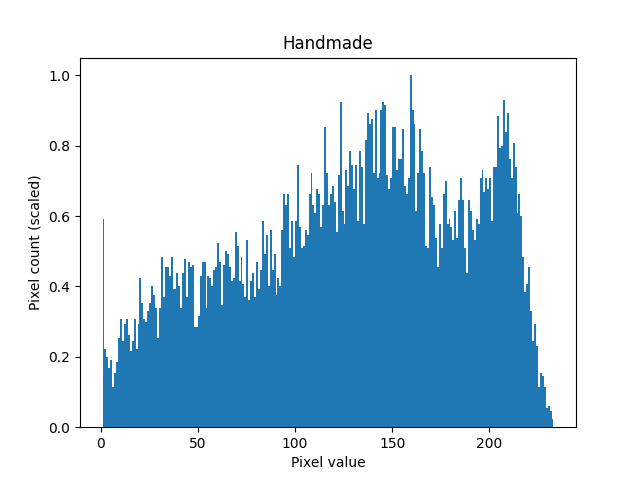
\includegraphics[width=0.7\columnwidth]{Immagini/handmade_scaled_hist.png}
%     \caption{Distribuzione Intensità dei pixel della segmentazione manuale}
%     \label{fig:distribuzione intensità dei pixel della segmentazione manuale}
% \end{figure}

% \begin{figure}[h!]
%     \centering
%     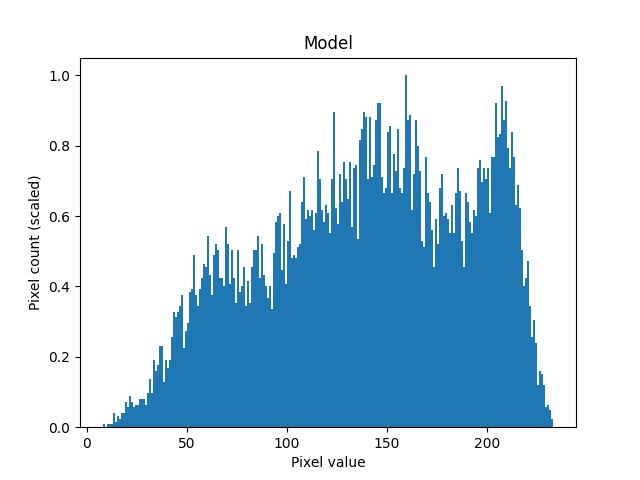
\includegraphics[width=0.7\columnwidth]{Immagini/model_scaled_hist.png}
%     \caption{Distribuzione Intensità dei pixel della segmentazione del modello}
%     \label{fig:distribuzione intensità dei pixel della segmentazione del modello}
% \end{figure}

\begin{figure}[h!]
    \centering
    \begin{minipage}{0.45\columnwidth}
        \centering
        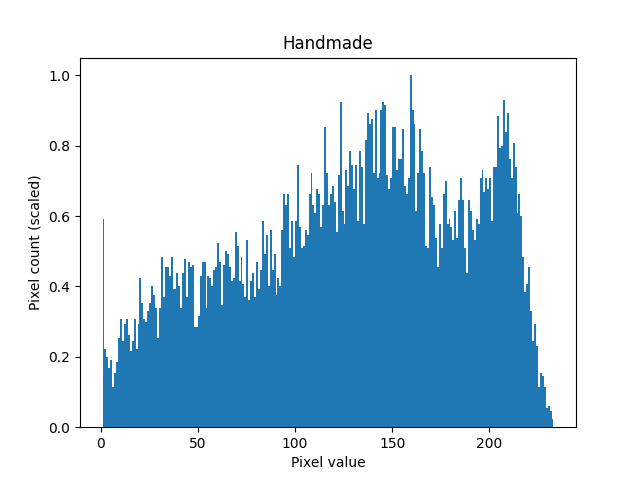
\includegraphics[width=\linewidth]{Immagini/handmade_scaled_hist.png}
        \caption{Distribuzione Intensità dei pixel della segmentazione manuale}
        \label{fig:distribuzione intensità dei pixel della segmentazione manuale}
    \end{minipage}
    \hfill
    \begin{minipage}{0.45\columnwidth}
        \centering
        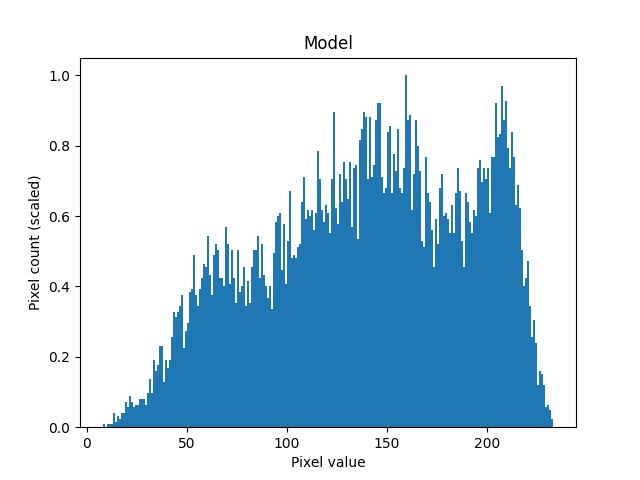
\includegraphics[width=\linewidth]{Immagini/model_scaled_hist.png}
        \caption{Distribuzione Intensità dei pixel della segmentazione del modello}
        \label{fig:distribuzione intensità dei pixel della segmentazione del modello}
    \end{minipage}
\end{figure}

\begin{figure}[h!]
    \centering
    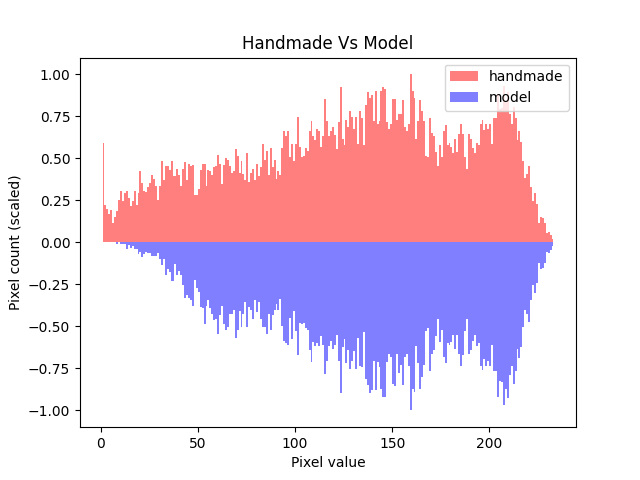
\includegraphics[width=0.7\columnwidth]{Immagini/handmade_vs_model_scaled.png}
    \caption{Confronto tra la segmentazione manuale e quella del modello}
    \label{fig:confronto tra la segmentazione manuale e quella del modello}
\end{figure}


Dai risultati qualitativi e quantitativi si pu\`o constatare che il modello ha una performance
molto promettente in quanto supera abbondantemente un'accuratezza del $90\%$ e pu\`o essere 
addestrato incrementando il numero d'immagini a disposizione. 

Non sono necessari ulteriori segmentazioni manuali ma si possono direttamente sfruttare
le nuove immagini raccolte, segmentarle mediante l'uso del modello e utilizzarle per l'addestramento.




% % section Addestramento (end)





% % chapter Risultati sperimentali (end)

% \chapter{Formattazione}\label{chapter:formattazione}
Prima di introdurre il capitolo si può scrivere una breve introduzione su ciò che si andrà ad affrontare.
In questo capitolo, per esempio, saranno presentati alcuni esempi di formattazione degli oggetti più comuni di una Tesi in informatica.


\section{Capitoli, Sezioni e Sottosezioni}\label{sec:cap_sec_subsec}
Capitoli, sezioni e sottosezioni devono essere usate appropriatamente e non sostituire elenchi puntanti.
In particolare, i Capitoli devono riguardare macro-argomenti della tesi; ad esempio \textbf{Background}, \textbf{Obiettivi}, \textbf{Progettazione/Implementazione} e \textbf{Risultati}.
Questi capitoli sono semplicemente una traccia bisogna adattare a seconda delle esigenze.

Le sezioni invece devono riguardare argomenti all'interno della macro-area definita dal capitolo.
Ad esempio se più tecniche sono state utilizzate durante la tesi si può suddividere il capitolo \textbf{Progettazione/Implementazione} in sezioni, ognuna riguardante una delle tecniche sperimentate.

Le sottosezioni infine si possono utilizzare per descrivere concetti distinti all'interno di ogni sezione, ognuno dei quali deve avere una sua identità.
Ogni sottosezione deve avere un motivo per essere definita e non semplicemente separare parti di uno stesso discorso, per quello c'è l'indentazione (doppio ``a capo'' per separare parti distinte dello stesso paragrafo e ``$\backslash\backslash$'' per separare due paragrafi).

\subsection{Esempio di sottosezione}\label{subsec:es_subsec}
\blindtext

\section{Esempi di Immagini}\label{sec:images}
Di seguito alcuni esempi di immagini.
Figura~\ref{fig:one} presenta una singola immagine con ancoraggio ``\textbf{ht}" che chiede al altex di lasciare la figura dove si trova, se possibile, e altrimenti di metterla in alto alla pagina.
Figura~\ref{fig:two} presenta una singola immagine con due sotto-figure con ancoraggio ``\textbf{ht}".
Figura~\ref{fig:three} presenta una singola immagine con tre sotto-figure con ancoraggio ``\textbf{H}" che forza l'immagine nel posto scelto dall'utente, questa opzione è sconsigliata a meno di necessità particolari.
Ogni volta che un'immagine è inserita è buona norma citarla nel testo, altrimenti l'immagine non avrebbe un chiaro significato.
Nel caso delle sotto-immagini si possono citare anche loro, ad esempio Figura~\ref{fig:lev1} è composta da altre due sotto-figure.
\begin{figure}[ht]
	\centering
	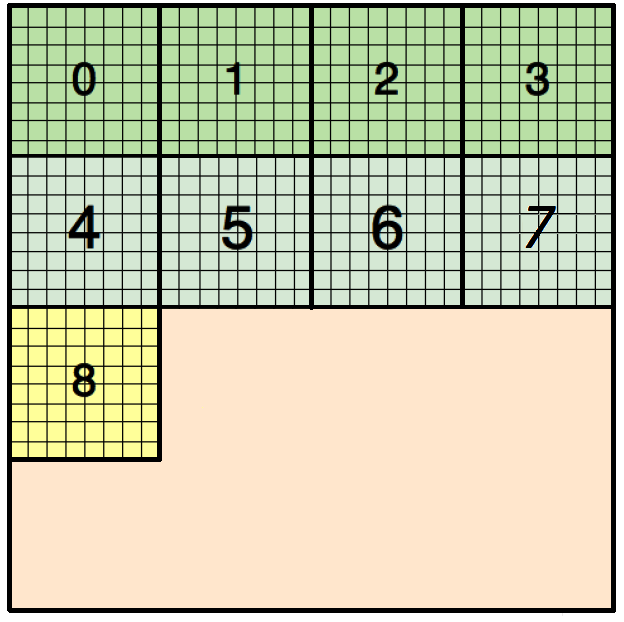
\includegraphics[width=0.3\textwidth]{Immagini/block_on_grid.png}
	\caption{Figura con singola immagine}
	\label{fig:one}
\end{figure}

\begin{figure}[ht]
	\centering
	\begin{subfigure}{0.3\textwidth}
		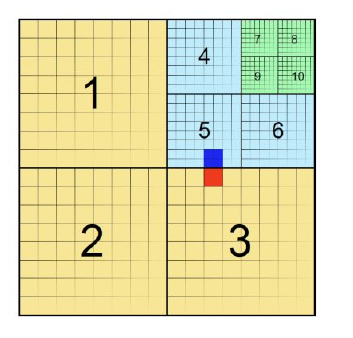
\includegraphics[width=1.0\textwidth]{Immagini/disoposizione_blocchi_fisica.png}
		\caption{Disposizione fisica dei blocchi}
	\end{subfigure}%
	\begin{subfigure}{0.3\textwidth}
		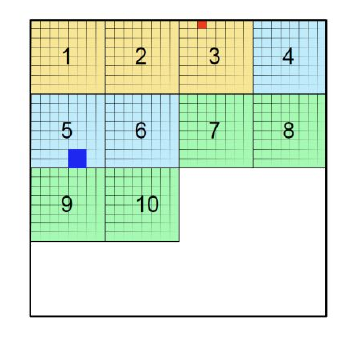
\includegraphics[width=1.0\textwidth]{Immagini/disoposizione_blocchi_logica.png}
		\caption{Disposizione logica dei blocchi}
	\end{subfigure}
	\caption{Figura con due immagini}
	\label{fig:two}
\end{figure}


\begin{figure}[H]
	\centering
	\begin{subfigure}{0.5\textwidth}
		\centering
		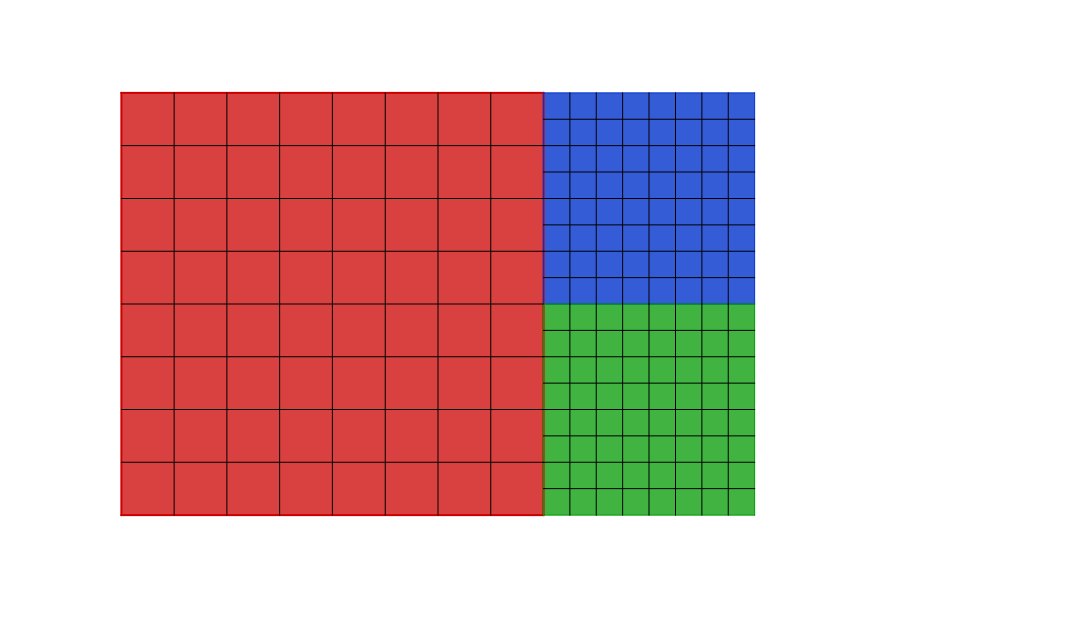
\includegraphics[width=0.7\linewidth]{Immagini/lev_less1.png}
		\caption{\textit{lev} = -1\newline}
		\label{fig:test1}
	\end{subfigure}%
	\begin{subfigure}{0.5\textwidth}
		\centering
		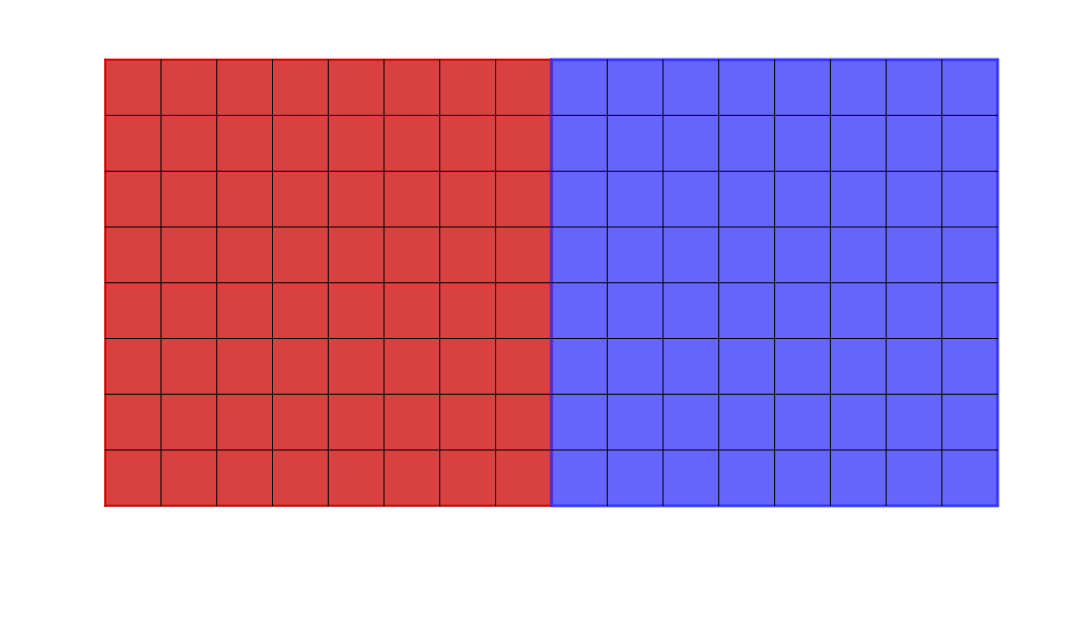
\includegraphics[width=0.7\linewidth]{Immagini/lev0.png}
		\caption{\textit{lev} = 0\newline}
		\label{fig:test2}
	\end{subfigure}
	\begin{subfigure}{0.7\textwidth}
		\centering
		\begin{subfigure}{0.5\textwidth}
			\centering
			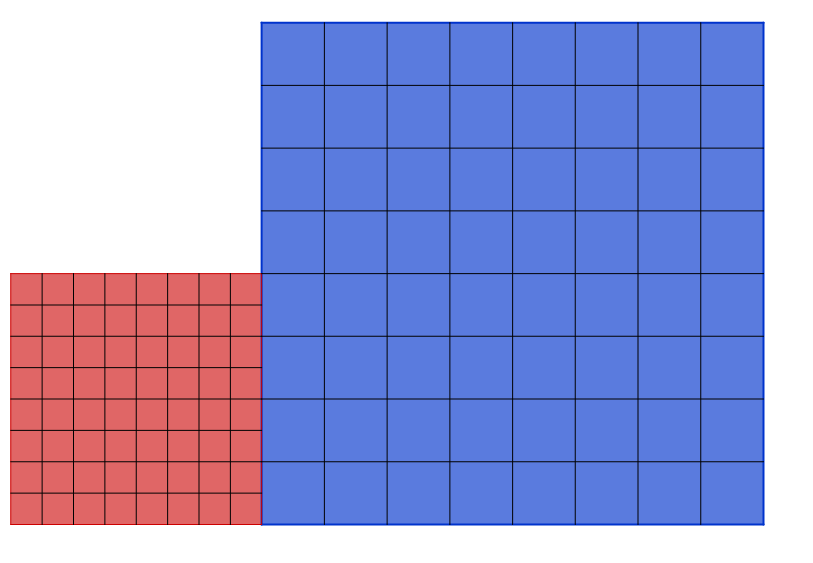
\includegraphics[width=0.5\linewidth]{Immagini/bloccomaggiore1.png}
		\end{subfigure}%
		\begin{subfigure}{0.5\textwidth}
			\centering
			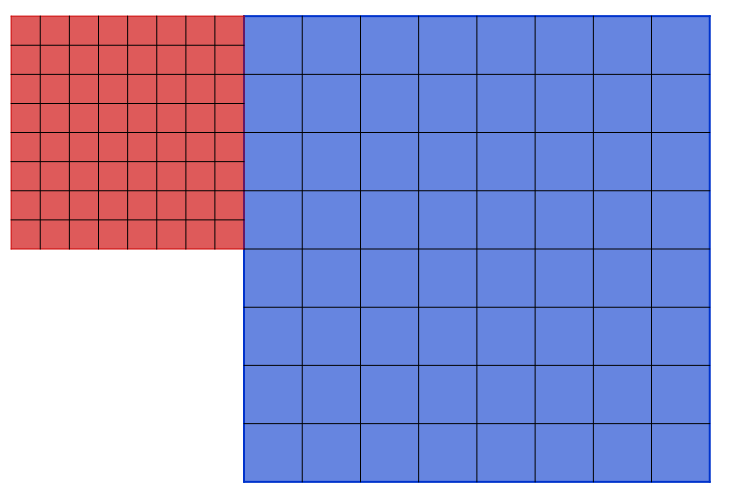
\includegraphics[width=0.5\linewidth]{Immagini/bloccomaggiore2.png}
		\end{subfigure}
		\caption{\textit{lev} = 1}
		\label{fig:lev1}
	\end{subfigure}
	\caption{Figura con tre immagini (di cui una composta da due sotto-immagini)}
	\label{fig:three}
\end{figure}

\section{Esempi di Codice e Misc.}\label{sec:code}
Alcuni esempi di codice, definizioni, tabelle e altro.

\begin{algorithm}[ht]
	\caption{Esempio di pseudo-codice}
	\label{alg:Prim_Mst}
	\begin{algorithmic}[1]
		\Statex
		\Function{MST-Prim}{grafo G, funzione\_peso $\omega$, nodo\_radice r}\\
		\State{\textit{Q}: coda di priorita contenente tutti i vertici in \textit{V}}
		\For{ogni \textit{u} $\in$ V(G)}
		\Let{\textit{u.key}}{$\infty$}
		\Let{\textit{u.}$\pi$}{\textit{NIL}} 
		\EndFor
		\Let{\textit{r.key}}{0}
		\Let{\textit{Q}}{\textit{V(G)}}
		\While{\textit{Q} $\neq$ 0}
		\Let{\textit{u}}{EXTRACT-MIN(\textit{Q})}
		\For{ogni \textit{v} $\in$ \textit{G.Adj[u]}}
		\If{$v \in Q$ and $\omega(u,v) < v.key$}
		\Let{\textit{v.key}}{$\omega(u,v)$}
		\Let{\textit{v.}$\pi$}{\textit{v}}
		\EndIf
		\EndFor
		\EndWhile
		\State \Return{}
		\EndFunction
	\end{algorithmic}
\end{algorithm}

\begin{minipage}{\textwidth}
\begin{lstlisting}[caption={Esempio di definizione struttura dati C++, ma non algoritmo},
	label={lst:block_struct}]
	struct Block
	{
		int id_block;
		char resolution;
		int id_subdomain;
		int key;
		bool in_other_subdomain;
		struct neigh_t neighbors[4];
	};
\end{lstlisting}
\end{minipage}



\begin{algorithm}[ht]
	\caption{Esempio di codice imperativo}
	\label{alg:my_prim_multi}
	\begin{algorithmic}[1]
		\Statex
		\Function{PRIM\_MULTI-MST}{roots\_list \textit{roots}, array\_Block \textit{adjacency\_list}}
		
		\State{\color{blue}{//Inizializzazione di tutti i vertici}}
		\For{ogni \textit{u} $\in$ \textit{adjacency\_list}}
		\Let{\textit{u.key}}{$\infty$}
		\Let{\textit{u.id\_subdomains}}{\textit{NIL}}
		\Let{\textit{u.in\_other\_subdomain}}{FALSE} 
		\EndFor
		
		\State{\color{blue}{//Inizializzazione di tutte le radici}}
		\Let{\textit{i}}{0}
		\For{ogni \textit{r} $\in$ \textit{roots}}
		\Let{\textit{r.key}}{0}
		\Let{\textit{r.id\_subdomains}}{\textit{i}}
		\Let{\textit{i}}{$i+1$}
		\EndFor
		\State{\textit{Q}: coda di priorita ordinata in base al campo 
			\textit{key}}
		\Let{\textit{Q}}{\textit{roots}}
		\Let{\textit{count}}{0}
		
		\While{count $<$ \textit{adjacency\_list.size}}
		\Let{\textit{u}}{EXTRACT-MIN(\textit{Q})}
		
		\If{!(\textit{u.in\_other\_subdomain})}
		\State{\color{blue}{//Essendo il minimo viene aggiunto definitivamente}}
		\Let{\textit{u.in\_other\_subdomain}}{TRUE}
		\State{\color{blue}{//Si analizzano i vicini}}
		\For{ogni \textit{v} $\in$ \textit{u.neighbors}}
		\State{\color{blue}{//In questo caso specifico il peso di ogni arco vale 1}}
		\If{$v \in adjacency\_list$ and ($u.key+1) < v.key$}
		\Let{\textit{v.key}}{$u.key+1$}
		\Let{\textit{v.subdomains}}{\textit{u.subdomains}}
		\Let{\textit{count}}{\textit{count} + 1}
		\EndIf
		\EndFor
		\EndIf
		\EndWhile
		\State \Return{}
		\EndFunction
	\end{algorithmic}
\end{algorithm}

\begin{algorithm}[ht]
	\caption{esempio di algoritmo in C++}
	\label{lst:genic_mpi}
	\begin{lstlisting}
		#include (*@\textquotedblleft@*)mpi.h"
		
		(*@~ ~ ~ ~\raisebox{-1pt}[0pt][0pt]{$\vdots$}@*)
		
		main(int argc, char** argv){
			
			(*@~ ~ ~ ~ ~ ~ ~ ~ ~ ~{\raisebox{-1pt}[0pt][0pt]{$\vdots$}}@*)
			
			//Nessuna chiamata a funzioni MPI prima di questa
			MPI_Init(&argc, &argv);
			
			(*@~ ~ ~ ~ ~ ~ ~ ~ ~ ~{\raisebox{-1pt}[0pt][0pt]{$\vdots$}}@*)
			
			MPI_Finalize();
			//Nessuna chiamata a funzioni MPI dopo questa
			
			(*@~ ~ ~ ~ ~ ~ ~ ~ ~ ~{\raisebox{-1pt}[0pt][0pt]{$\vdots$}}@*)
		}	
	\end{lstlisting}
\end{algorithm}

\begin{defn}[Esempio di Definizione]
	Un piccolo esempio di definizione
\end{defn}

\begin{table}[ht]
	\centering
	\resizebox{0.99\linewidth}{!}{
		\begin{tabular}{||c||c|c|c|c|c|c|c|c|c|c||}
			\hhline{|t:=:t:==========:t|}
			CT scan &\phantom{00}01\phantom{00}&\phantom{00}02\phantom{00}&\phantom{00}03\phantom{00}&\phantom{00}04\phantom{00}&\phantom{00}05&\phantom{00}06\phantom{00}&\phantom{00}07\phantom{00}&\phantom{00}08\phantom{00}&\phantom{00}09\phantom{00}&\phantom{00}10\phantom{00} \\
			\hhline{|:=::==========:|}
			Input arteries (n.) &66&175&76&134&198&172&154&108&91&65 \\
			\hhline{||-||----------||}
			Labeling time (s)&19.13&87.38&26.11&47.08&90.89&356.95&303.77&91.95&16.01&21.88 \\
			\hhline{||-||----------||}
			Grounding time (s)&9.76&52.45&9.57&22.88&70.34&47.52&37.44&17.98&10.61&8.04 \\
			\hhline{||-||----------||}
			Optimum time (s)&6.66&31.05&14.67&20.63&15.2&29.17&54.71&61.03&4.28&7.24 \\
			\hhline{|b:=:b:==========:b|}
		\end{tabular}
	}
	\vspace*{2mm}
	\caption{Esempio di tabella}
	\label{tab:perf}
\end{table}


\section{Citazioni}
Durante la scrittura della Tesi è necessario fornire i riferimenti bibliografici che hanno permesso la stesura della tesi stessa.
Questo si ottiene semplicemente tramite l'utilizzo del comando ``cite'' che prende come argomento la label di una delle entry nel file .bib.
Quindi per citare una qualunque fonte, ad esempio ``Artificial Intelligence - A Modern Approach", si può fare \cite{modernApproach} ($\backslash\text{cite}\{\text{modernApproach}\}$).
Questo leggerà la referenza nel file .bib che ha come label ``cormen".
Per citare più riferimenti contemporaneamente basta sperare le varie labels con una virgola come segue \cite{gelfond1998action,modernApproach,durfee1999distributed,de2003resource,allen2009complexity,bernstein2002complexity}.
Le reference non citate non appariranno in bibliografia.
\href{https://dblp.uni-trier.de/}{dblp} e \href{https://scholar.google.com/}{Google Scholar} sono siti nei quali estrarre la reference per bibtex per un lavoro di cui si conosce solo il titolo, ad esempio.
% \chapter{Background}\label{chapter:background}
\Blindtext %Dummy Text - remove
\Blindtext %Dummy Text - remove
% \chapter{Obbiettivi}\label{chapter:obbiettivi}
\Blindtext %Dummy Text - remove
% \chapter{Progettazione}\label{chapter:progettazione}
\Blindtext
% \chapter{Risultati}\label{chapter:res}
\Blindtext %Dummy Text - remove
%
%
%%%% Le Conclusioni
\pagestyle{plain}
% \chapter*{Conclusione} %Se si cambia il Titolo cambiare anche la riga successiva così che appia corretto nell'conclusione
\addcontentsline{toc}{chapter}{Conclusione} %Per far apparire Introduzione nell'indice (Il nome deve rispecchiare quello del chapter)
Conclusione che riassume il lavoro svolto ed eventuali lavori futuri.

\blindtext %Dummy Text - remove
\blindtext %Dummy Text - remove
%
%%%% La bibliografia
\bibliographystyle{apalike} %{plain} -- Scegliere lo stile preferito
\cleardoublepage
\addcontentsline{toc}{chapter}{\bibname}
\bibliography{./Bibliografia}
%
% \chapter*{Ringraziamenti}
\Blindtext %Dummy Text - remove
%
% Le appendici
\appendix
% \chapter{Appendice di Esempio}
\Blindtext
%
\end{document}
